%-*-latex-*-
\sectionthree{Array trees}
\begin{python0}
from solutions import *; clear()
\end{python0}

You have already seen trees using nodes which are dynamically
allocated in the memory heap.
Actually, it's possible to build trees using array!
I'll just explain how to do this for the case of binary trees.


\begin{center}
\begin{tikzpicture}[>=triangle 60,shorten >=0.5pt,node distance=2cm,auto,initial text=, double distance=2pt]
\node[state] (A) at (  3,  0) {$A$};
\node[state] (B) at (  6,  0) {$B$};
\node[state] (S) at (  0, -2) {$S$};
\node[state] (C) at (  3, -4) {$C$};

\path[->]
(A) edge [bend left=0,pos=0.5,above] node {} (B)
(A) edge [bend left=0,pos=0.5] node {} (C)
(S) edge [bend left=0,pos=0.5,above] node {} (A)
(S) edge [bend left=0,pos=0.5,above] node {} (C)

;
\end{tikzpicture}
\end{center}
    


I can lay it out in an array like this:

%-*-latex-*-
\begin{Verbatim}[frame=single,fontsize=\small]
[student@localhost discrete-probability] python discrete-probrobability/game2.py
python: can't open file 'discrete-probrobability/game2.py': [Errno 2] No such fi
le or directory
\end{Verbatim}



In other words, traverse the tree using breadth-first left-to-right
and put a value into the array as you see visit the value in the tree.

The above tree is complete.
What if it's not?

One option is to use a sentinel to denote the
fact that an array element is not filled with a node value.
For instance, say I have this tree:

%-*-latex-*-
{\footnotesize \begin{Verbatim}[frame=single,fontsize=\small]
[student@localhost discrete-probability] python tossfaircoin2.py
experiment 0 ... outcome: TAIL
experiment 1 ... outcome: TAIL
experiment 2 ... outcome: TAIL
experiment 3 ... outcome: TAIL
experiment 4 ... outcome: TAIL
experiment 5 ... outcome: TAIL
experiment 6 ... outcome: HEAD
experiment 7 ... outcome: TAIL
experiment 8 ... outcome: TAIL
experiment 9 ... outcome: TAIL
experiment 10 ... outcome: TAIL
experiment 11 ... outcome: HEAD
experiment 12 ... outcome: HEAD
experiment 13 ... outcome: TAIL
experiment 14 ... outcome: HEAD
experiment 15 ... outcome: TAIL
experiment 16 ... outcome: TAIL
experiment 17 ... outcome: HEAD
experiment 18 ... outcome: HEAD
experiment 19 ... outcome: TAIL
number of experiments: 20
number of heads: 6
number of tails: 14
probability of getting head: 0.3
probability of getting tail: 0.7
\end{Verbatim}
}


\begin{console}
12094
\end{console}


Another option is to include a delete flag
for each value in the array.
If the element of the array represents a node,
the delete flag is false.
However if the element of the array does not hold a node,
then the delete flag is set to true.



Of course a tree is not just a collection of data.
It's a graph.
You have to describe edges, i.e., you must
connect the values.
How can we do that?
Well note that the left child of node with value \verb!5! is 
the node with value \verb!2!:

\begin{center}
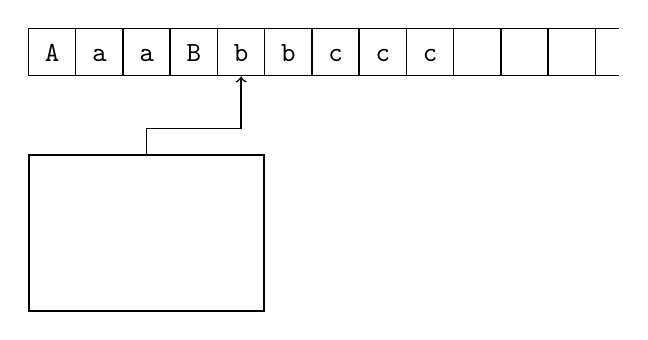
\begin{tikzpicture}

\draw (0.3, 0.3)
  node[draw, line width=0.02cm, , color=black,
       rounded corners=0cm, inner sep=0cm] {

\begin{minipage}[t][0.6cm]{0.6cm}
\mbox{}

\end{minipage}

};\draw (0.3, 0.3) node[color=black] {{\vphantom{AaaBbbccc$\BLANK$$\BLANK$$\BLANK$}\texttt{A}}};
\draw (0.8999999999999999, 0.3)
  node[draw, line width=0.02cm, , color=black,
       rounded corners=0cm, inner sep=0cm] {

\begin{minipage}[t][0.6cm]{0.6cm}
\mbox{}

\end{minipage}

};\draw (0.8999999999999999, 0.3) node[color=black] {{\vphantom{AaaBbbccc$\BLANK$$\BLANK$$\BLANK$}\texttt{a}}};
\draw (1.5, 0.3)
  node[draw, line width=0.02cm, , color=black,
       rounded corners=0cm, inner sep=0cm] {

\begin{minipage}[t][0.6cm]{0.6cm}
\mbox{}

\end{minipage}

};\draw (1.5, 0.3) node[color=black] {{\vphantom{AaaBbbccc$\BLANK$$\BLANK$$\BLANK$}\texttt{a}}};
\draw (2.0999999999999996, 0.3)
  node[draw, line width=0.02cm, , color=black,
       rounded corners=0cm, inner sep=0cm] {

\begin{minipage}[t][0.6cm]{0.6cm}
\mbox{}

\end{minipage}

};\draw (2.0999999999999996, 0.3) node[color=black] {{\vphantom{AaaBbbccc$\BLANK$$\BLANK$$\BLANK$}\texttt{B}}};
\draw (2.7, 0.3)
  node[draw, line width=0.02cm, , color=black,
       rounded corners=0cm, inner sep=0cm] {

\begin{minipage}[t][0.6cm]{0.6cm}
\mbox{}

\end{minipage}

};\draw (2.7, 0.3) node[color=black] {{\vphantom{AaaBbbccc$\BLANK$$\BLANK$$\BLANK$}\texttt{b}}};
\draw (3.3, 0.3)
  node[draw, line width=0.02cm, , color=black,
       rounded corners=0cm, inner sep=0cm] {

\begin{minipage}[t][0.6cm]{0.6cm}
\mbox{}

\end{minipage}

};\draw (3.3, 0.3) node[color=black] {{\vphantom{AaaBbbccc$\BLANK$$\BLANK$$\BLANK$}\texttt{b}}};
\draw (3.9000000000000004, 0.3)
  node[draw, line width=0.02cm, , color=black,
       rounded corners=0cm, inner sep=0cm] {

\begin{minipage}[t][0.6cm]{0.6cm}
\mbox{}

\end{minipage}

};\draw (3.9000000000000004, 0.3) node[color=black] {{\vphantom{AaaBbbccc$\BLANK$$\BLANK$$\BLANK$}\texttt{c}}};
\draw (4.5, 0.3)
  node[draw, line width=0.02cm, , color=black,
       rounded corners=0cm, inner sep=0cm] {

\begin{minipage}[t][0.6cm]{0.6cm}
\mbox{}

\end{minipage}

};\draw (4.5, 0.3) node[color=black] {{\vphantom{AaaBbbccc$\BLANK$$\BLANK$$\BLANK$}\texttt{c}}};
\draw (5.1, 0.3)
  node[draw, line width=0.02cm, , color=black,
       rounded corners=0cm, inner sep=0cm] {

\begin{minipage}[t][0.6cm]{0.6cm}
\mbox{}

\end{minipage}

};\draw (5.1, 0.3) node[color=black] {{\vphantom{AaaBbbccc$\BLANK$$\BLANK$$\BLANK$}\texttt{c}}};
\draw (5.699999999999999, 0.3)
  node[draw, line width=0.02cm, , color=black,
       rounded corners=0cm, inner sep=0cm] {

\begin{minipage}[t][0.6cm]{0.6cm}
\mbox{}

\end{minipage}

};\draw (5.699999999999999, 0.3) node[color=black] {{\vphantom{AaaBbbccc$\BLANK$$\BLANK$$\BLANK$}\texttt{$\BLANK$}}};
\draw (6.299999999999999, 0.3)
  node[draw, line width=0.02cm, , color=black,
       rounded corners=0cm, inner sep=0cm] {

\begin{minipage}[t][0.6cm]{0.6cm}
\mbox{}

\end{minipage}

};\draw (6.299999999999999, 0.3) node[color=black] {{\vphantom{AaaBbbccc$\BLANK$$\BLANK$$\BLANK$}\texttt{$\BLANK$}}};
\draw (6.899999999999999, 0.3)
  node[draw, line width=0.02cm, , color=black,
       rounded corners=0cm, inner sep=0cm] {

\begin{minipage}[t][0.6cm]{0.6cm}
\mbox{}

\end{minipage}

};\draw (6.899999999999999, 0.3) node[color=black] {{\vphantom{AaaBbbccc$\BLANK$$\BLANK$$\BLANK$}\texttt{$\BLANK$}}};\draw[line width=0.02cm,black] (7.1999999999999975,0.6) to  (7.499999999999998,0.6);
\draw[line width=0.02cm,black] (7.1999999999999975,0.0) to  (7.499999999999998,0.0);

\draw (1.5, -2.0)
  node[draw, line width=0.02cm, , color=black,
       rounded corners=0cm, inner sep=0cm] {

\begin{minipage}[t][1.98cm]{2.98cm}
\mbox{}

\end{minipage}

};\draw[line width=0.02cm,black,->] (1.5,-1) to  (1.5,-0.67) to  (2.7,-0.67) to  (2.7,-0.01);
\end{tikzpicture}

\end{center}



You notice that the index of \verb!5! is 0 and the index of 
\verb!2! is 1.
Also, note that the left child of \verb!2! is \verb!6!
which is at index 3.
The left child of \verb!0!, which is at index 2, is \verb!8!,
which is at index 5.
For all the above cases,
you notice the the left child of the value at index $i$
is at index $2i + 1$.
Correct?

Do you also notice that the value at index $i$, the
right child is at index $2i + 2$?

Going to the parent is easy.
If you look at the value at index $j$,
then you have the followning fact:
\begin{tightlist}
\li If $j$ is odd, then the parent is at index $(j - 1) / 2$.
Why? Because in this case $j = 2i + 1$ and I want $i$.
This is just $i = (j - 1) / 2$.
\li If $j$ is even, then the parent is at index $(j - 2)/ 2$.
Why? Because in this case $j = 2i + 2$ and I want $i$.
Of course $i = (j - 2) / 2$.
Note that using integer division, this is the same as
$(j - 1) / 2$.
Correct?
\end{tightlist}

Let me summarize:
\begin{tightlist}
\li The left child of the node at index $i$ is at index $2i+1$.
\li The right child of the node at index $i$ is at index $2i+2$.
\li The parent of the node at index $j$ is at index $(j - 1)/2$
    where the division above is integer division.
\end{tightlist}


\begin{Verbatim}[frame=single]
ALGORITHM: left
INPUT:     i - an index in an array say x
OUTPUT:    index where x[index] is the left child of x[i]

return 2 * i + 1
\end{Verbatim}
\begin{Verbatim}[frame=single]
ALGORITHM: right
INPUT:     i - an index in an array say x
OUTPUT:    index where x[index] is the right child of x[i]

return 2 * i + 2
\end{Verbatim}
\begin{Verbatim}[frame=single]
ALGORITHM: parent
INPUT:     j - an index in an array say x
OUTPUT:    index where x[parent(i)] is the parent of x[i]

return (j - 1) / 2
\end{Verbatim}

So if I have a complete binary tree where
the missing nodes are all on the right of the last level,
I can use an array to represent the tree
and the \verb!left!, \verb!right!, and \verb!parent!
functions
can be used to form parent-child
between the values of the array.

Sometimes when you read books on array trees, you will see that
usually first element of the array, i.e., the element at
index 0 is not used.
In that case you have the following:
\begin{tightlist}
\li The left child of the node at index $i$ is at index $2i$.
\li The right child of the node at index $i$ is at index $2i+1$.
\li The parent of the node at index $j$ is at index $j / 2$
    where the division above is integer division, i.e., 
    mathematically it should be 
    $\floor{j / 2}$
\end{tightlist}
So be careful!

Whereas in the case of trees built with nodes in the heap
and therefore we need pointers hold address values to the nodes,
in the case of array trees, I will be using integer variables
containing index values.

% asdfasdf

\begin{ex} 
  \label{ex:some-decision1}
  \tinysidebar{\debug{exercises/{empty0/question.tex}}}
  \solutionlink{sol:some-decision1}
  \qed
\end{ex} 
\begin{python0}
from solutions import *
add(label="ex:some-decision1",
    srcfilename='exercises/some-decision1/answer.tex') 
\end{python0}


\newpage
\begin{ex}
How would you build a $k$--ary tree using 
arrays?
Draw a $3$--ary tree with about 20 nodes (with integer values).
\begin{tightlist}
  \item If \texttt{i} is an index, what is index of the $d$--th child?
  \item If \texttt{j} is an index, what is index of the parent?
\end{tightlist}
\qed
\end{ex}
 
